This section contains all software requirements both functional and non-functional.
A requirement has the following properties:
\begin{itemize}
	\item[\bf{Requirement ID}] Uniquely identifies requirement within all TaskList documents.
	\item[\bf{Title}] Gives the requirement a symbolic name.
	\item[\bf{Description}] The definition of the requirement.
	\item[\bf{Priority}] Defines the order in which the requirements should be implemented. Priorities are designated from highest to lowest.
	Possible values are 1 (first to implement), 2 and 3 (last to implement).
	\item[\bf{Risk}] Specifies risk of not implementing this requirement. It shows how the particular requirement is critical to the system.
	there are the following risks levels and associated impact to the system if the requirement is not implemented or implemented incorrectly.
		\begin{itemize}
			\item {\bf Critical (C)}  will break the main functionality of the system. The system can not be used if this requirement is not implemented.
			\item {\bf High (H)} will impact the main functionality of the system. Some function of the system could be inaccessible, but the 
			system can be generally used.
			\item {\bf Medium (M)} will impact some systems features, but not the main functionality. System can be used with some limitation.
			\item {\bf Low (L)} the system can be used without limitation, but with some workarounds.

		\end{itemize}

  \end{itemize}


\subsection{Functional Requirements}
\label{requirements:functional}

\begin{requirement}{Introducing Tasks}
    \desc{The system shall provide the user with the capability of adding a Task in Tomboy Notes.}
    \priority{1}
    \riskref{C}
\end{requirement}

\begin{requirement}{Grouping Tasks together}
    \desc{The system shall provide the user with the possibility to group certain tasks together in a list called a task list.}
    \priority{1}
    \riskref{C}
\end{requirement}

\begin{requirement}{Priorities for Tasks}
    \desc{The user can optionally add priorities to individual tasks and task lists.}
    \priority{1}
    \riskref{H}
\end{requirement}

\begin{requirement}{Due Dates for Tasks}
    \desc{The user can optionally add due dates to individual tasks and task lists.}
    \priority{1}
    \riskref{H}
\end{requirement}

\begin{requirement}{Subtasks}
    \desc{The system provides the user with the ability to model a task as a complex task consisting of possibly multiple subtasks.}
    \priority{1}
    \riskref{H}
\end{requirement}

\begin{requirement}{Exporting Tasks}
    \desc{The system provides a function to export all tasks in all notes and their corresponding information in an XML format.}
    \priority{3}
    \riskref{L}
\end{requirement}


    \subsubsection{Entity Diagram}
    The following diagram shows all defined entities from the requirements above and their relations.
    As we can see a Task is basically modeled as a string and - if its a more complex task - can link to other notes.
    \begin{figure}[h]
    	% TODO remove the grey licensing text in the diagram by using the software with a valid license key
      % I don't think that is possible without paying -> Just export it to pic with some dummy elements above and cut it in GIMP or something
	    \centering
        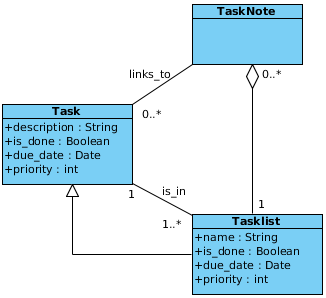
\includegraphics[width=0.5\textwidth]{graphics/entity_diagram.png}
        \caption{TaskList entities and relations}
        \label{entities_relations}
    \end{figure}
    
    This diagram does not define classes that must be implemented in software, but just the common entities



    \subsubsection{User Interface} %Jan
    \label{requirements:interfaces:user}

    \begin{requirement}{Create Task List}
      \desc{The user shall be able to create a new task list with a button or a shortcut text, like ``[]''. These lists expand automatically and contain individual tasks that can be marked as done.}
      \priority{1}
      \riskref{C}
    \end{requirement}

    \begin{requirement}{Edit Task List}
      \desc{The user can add, remove and change single task list items by directly editing the task list in the note itself.}
      \priority{1}
      \riskref{H}
    \end{requirement}

    \begin{requirement}{Due date visualization}
      \desc{The user should be able to set / change the due date for a task directly in the corresponding Tomboy note. 
      The system shall visualize to the user when items are near or even over their due date.}
      \priority{2}
      \riskref{M}
    \end{requirement}
    
    \begin{requirement}{Priority visualization}
      \desc{The user should be able to change the priority for a task directly in the corresponding Tomboy note. 
      The system shall visualize to the user the priority of a task and how important the task is in relation to other tasks in the same task list.}
      \priority{2}
      \riskref{M}
    \end{requirement}

    \begin{requirement}{Create Subtasks}
      \desc{The user can optionally create a task consisting of one or multiple other task lists considered as sub tasks for this particular task.}
      \priority{1}
      \riskref{H}
    \end{requirement}

    \begin{requirement}{Show / hide completed Tasks}
      \desc{The user gets various possibilities to handle completed tasks. He can show them crossed out, he can hide them, and he can show them after the completed tasks. }
      \priority{2}
      \riskref{M}
    \end{requirement}

    \begin{requirement}{Reorder Task Lists}
      \desc{The user has the possibility to order the task lists according to various criteria, like due date, priority, date added etc.}
      \priority{2}
      \riskref{L}
    \end{requirement}

    \begin{requirement}{Filter Notes}
      \desc{The user can query for a list of notes by setting some constraints which involve searching for notes who have unfinished or contain 
      tasks which are over their corresponding due date.}
      \priority{2}
      \riskref{M}
    \end{requirement}


	\subsubsection{Software Interfaces}
	\label{requirements:interfaces:software}
        %TODO => export (xml, evolution, tasque, ...)
        %     => Tomboy (save, ...)


	%\subsubsection{Communication Interfaces}
	%\label{requirements:interfaces:communication}

    \subsubsection{Supported Operating Systems}
    \label{requirements:os}
    \begin{requirement}{Platform independance}
      \desc{The Addin will work on any oerating system with a working installation of Tomboy (as defined in ?)}
      \priority{2}
      \riskref{M}
%TODO: where is this defined, anyway? (Version etc)
    \end{requirement}

\subsection{Nonfunctional Requirements}
\label{requirements:nonfunctional}

    \subsubsection{Licensing Requirements}
    \label{requirements:nonfunctional_start}
    \label{requirements:license}
    %TODO: Not sure this is really necessary!
    \begin{requirement}{license compliance}
      \desc{The project will comply to any restrictions imposed by Tomboy/GNOME licensing.}
      \priority{2}
      \riskref{M}
    \end{requirement}


    \subsubsection{Language}
    \label{requirements:language}
    \begin{requirement}{Default language}
      \desc{All system messages, texts, log entries and help documentation must by default be in English.}
      \priority{1}
    \end{requirement}

   
    \begin{requirement}{Translations}
      \desc{The Addin will integrate the built in language support and will therefore enable anyone being capable of writing Tomboy/Gnome translations to add additional language translations to the project}
    \end{requirement}

    \begin{requirement}{Interface Requirement}
      \desc{insert description}
      \priority{1}
      \riskref{C}
    \end{requirement}


    %\subsection{Performance Requirements}
    %\label{requirements:performance}

    \subsubsection{Design Constraints}
    \label{requirements:constraints}

    \begin{requirement}{Standard compliance}
      \desc{The project will be seen as part of Tomboy and will therefore comply to any existing standards and regulations imposed by Tomboy itself or the GNOME project}
      \priority{2}
      \riskref{L}
    \end{requirement}

    % => modules (textbuffer, note gui, notes window gui)
    % I don't really see this being a design constraint (constraint = Auflage/Bedingung) - Gabriel

    % -- I don't think this should be called this way. better have concrete subsubsections e.g. reliability (see below) - Gabriel
    %\subsubsection{Quality Requirements}
    %\label{requirements:quality}
    
    \subsubsection{Reliability}
    \label{requirements:reliability}
    \begin{requirement}{}  
    \end{requirement}
    % => Bugs, unit tests

    %\subsection{Other Requirements}
    %\label{requirements:other}

    \label{requirements:nonfunctional_end}
